% ------------------------------------------------------------------------
% file `revisions-exercise-10-solution-body.tex'
%   in folder `xsim/'
%
%     solution of type `exercise' with id `10'
%
% generated by the `solution' environment of the
%   `xsim' package v0.21 (2022/02/12)
% from source `revisions' on 2022/11/30 on line 267
% ------------------------------------------------------------------------
  \begin{enumerate}
    % \item 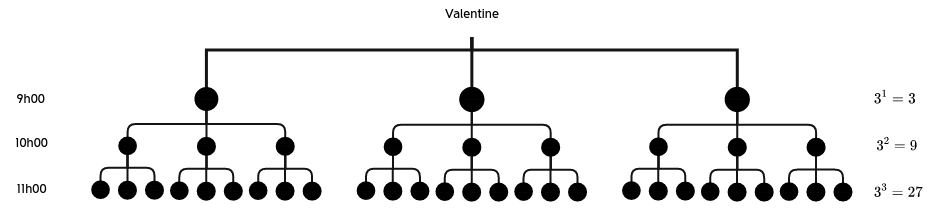
\includegraphics[width=\linewidth, valign=t]{img/rumeur.png}\par En suivant cette logique :
    % \begin{itemize}[label=\faIcon{caret-right}]
    %   \item à 14 h 00, $3^6=729$ personnes mises au courant
    %   \item à 19 h 00, $3^9=\num{19 683}$ personnes mises au courant
    % \end{itemize}

    % \item $\num{10000}\cdot 365\cdot 20 = 7,3\cdot 10^7$\par
    % Une jeune fille de 20 ans aura cligné $7,3\cdot 10^7$ fois depuis sa naissance.

    % \item Déterminons le volume de la plage en $\mathrm{mm^3}$. Pour cela convertissons nos grandeurs en mm.
    % \begin{itemize}[label=\faIcon{caret-right}]
    %   \item $\SI{1}{m} = \SI{1000}{mm} = 10^3~\mathrm{mm}$
    %   \item $\SI{5}{m} = \SI{5000}{mm} = 5 \cdot 10^3~\mathrm{mm}$
    %   \item $\SI{20}{km} = \SI{20000000}{mm} = 2 \cdot 10^7~\mathrm{mm}$
    % \end{itemize}
    % On détermine alors le volume de la plage, \[V_{plage} = 10^3~\mathrm{mm}\cdot 5 \cdot 10^3~\mathrm{mm} \cdot 2 \cdot 10^7~\mathrm{mm} = 10^{14}~\mathrm{mm^3}.\]
    % Nous savons que \SI{1}{mm^3} contient 10 grains de sables, on en déduit donc que la plage contient $10^{15}$ grains de sables.
    \item À 14 h 00, $3^6=729$ personnes mises au courant.\par
          À 19 h 00, $3^9=\num{19 683}$ personnes mises au courant.
    \item $7,3\cdot 10^7$.
    \item $10^{15}$ grains de sables.
    \item \SI{62}{cm}.
    \item $2,5\cdot 10^{13}$ globules rouges.
    \item Mercure < Mars < Vénus < Terre < Uranus < Jupiter.
  \end{enumerate}
